\chapter{Manual tweaks} \label{sec:manualtweaks}

First is required to bring the folder create by su2rad in the project folder of the TRNSYS simulation, and rename the folder Zone{\color{red} N} where {\color{red} N} is a positive integer number that define the zone analysed.\\
In figure \ref{img4:zone1} is shown an example of how locate the folder in the right place. The integer number that identifies the zone is the same number that has to be defined in Type's control panel under the input \textit{ZoneID}.
\begin{figure}[h]
\centering
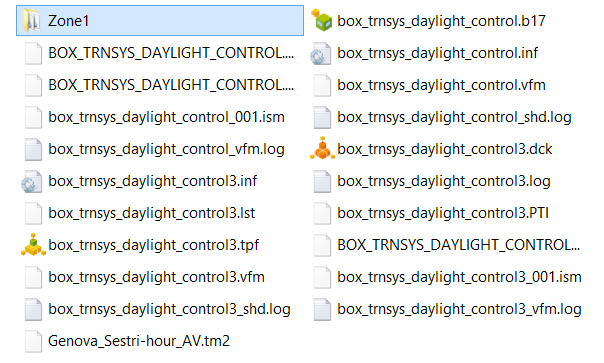
\includegraphics[width=0.7\textwidth]{zone1}
\caption{\label{img4:zone1} Positioning of the Radiance simulation folder in the TRNSYS project folder}
\end{figure}

Within the folder Zone1 is then necessary creating some folders: 
\begin{itemize}
\renewcommand{\labelitemi}{\tiny$\blacksquare$}
\item {\color{blue} data}, it will contain the matrices for the calculation, the file with the sensors grid and another subfolder:
\subitem{\tiny$\blacksquare$} {\color{blue} bsdf}, it will contain the bsdf data listed with integer numbers
\item {\color{blue} temp}, it will contain temporary files create during the matrices generation
\item {\color{blue} window}, it will contain the windows in the scene and a new file called win.vd
\end{itemize}

And deleting some other unused folder:
\begin{itemize}
\renewcommand{\labelitemi}{\tiny$\blacksquare$}
\item ambfiles
\item images
\item logfiles
\item octrees
\item skies
\end{itemize}

In order to make available the input data for TypeDLT it is necessary to modify some files generated by SketchUp and to create a new one, which will collect all the windows in the scene. Use a simple text editor to make these changes.\\
The 3PM requires that the windows in the scene are a secondary light source, so that the user has to change the windows material in glow material, see three-phase method tutorial for in-depth analysis. To do this the user has to open the rad file containing the window/windows geometries and add in the heading of this file the glow material definition paying attention to correspond the modifier of the geometry with the ID of the glow material as shown in figure \ref{img4:winglow}. Figure \ref{img4:wingroup} shows the case of a group windows. Then, move the window\_south.rad file from the "objects" folders to the "window" folder.

\begin{figure}[h] 
\centering
  \subfigure[]{% 
    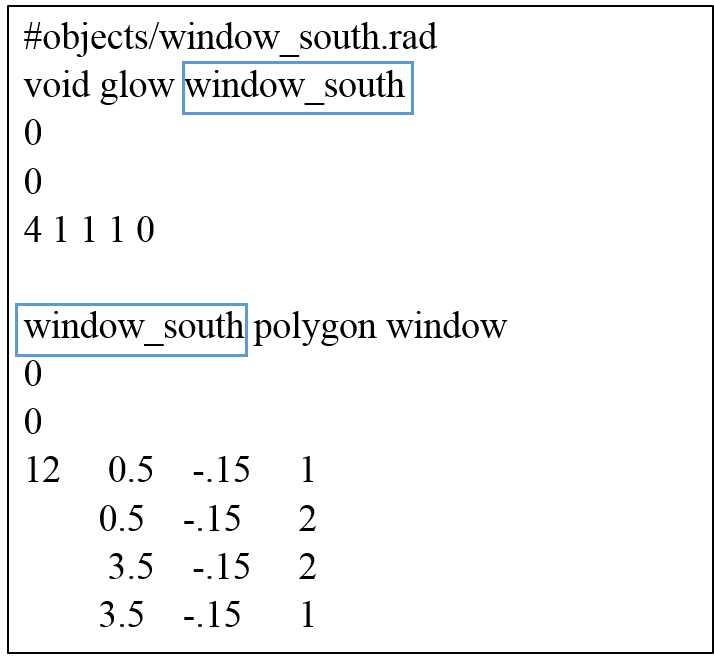
\includegraphics[width=.35\textwidth]{win} \label{img4:win} 
  }
  \subfigure[]{% 
    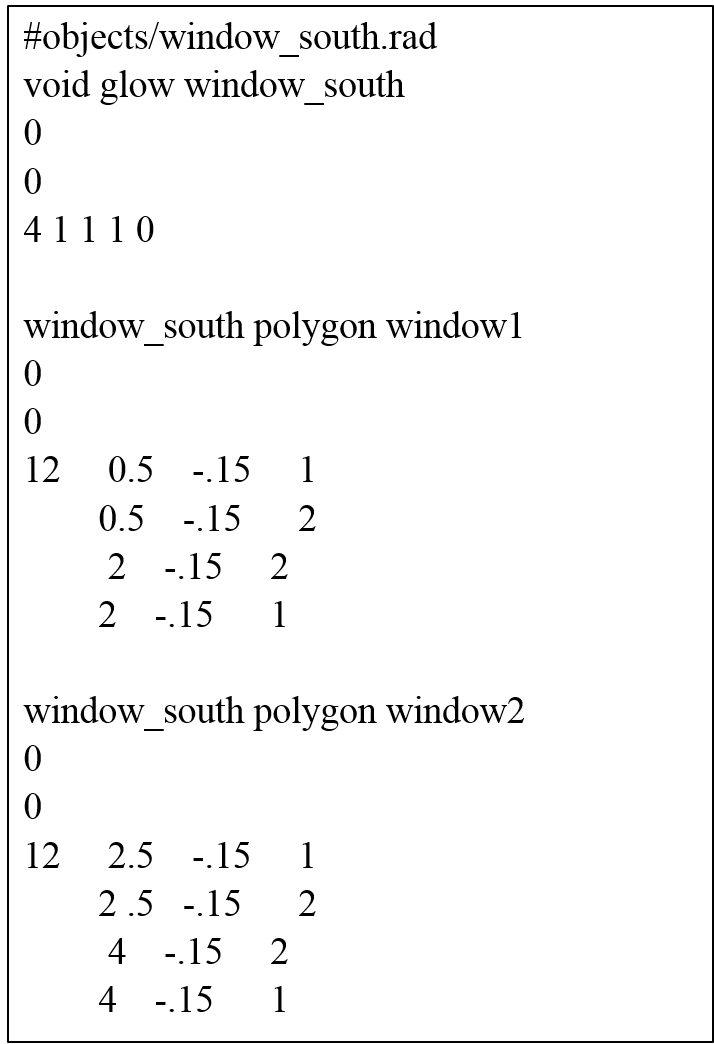
\includegraphics[width=.35\textwidth]{wingroup} \label{img4:wingroup} 
  } 
  \caption{\label{img4:winglow} Window file modified with the glow material for one window \ref{img4:win} and a group of two windows \ref{img4:wingroup}}
\end{figure}

A new file called {\color{blue} win.vd} has to be created within the "window" folder. In this new file insert the number of windows/group of windows and the  list of this windows/group of windows following a specific format: window modifier, view direction (vd) and view up (vp). The view direction is the window normal vector facing toward the outside of the room, the view up is the window up vector, vd and vu are always orthogonal. Figure \ref{img4:windoworient} shows how to choose vd and vu from a sample geometry in which there is a window facing south. It is also shown how to report these information in the win.vd file for a window with modifier window\_south.

\begin{figure}[H]
\centering
\begin{minipage}[c]{0.6\linewidth}
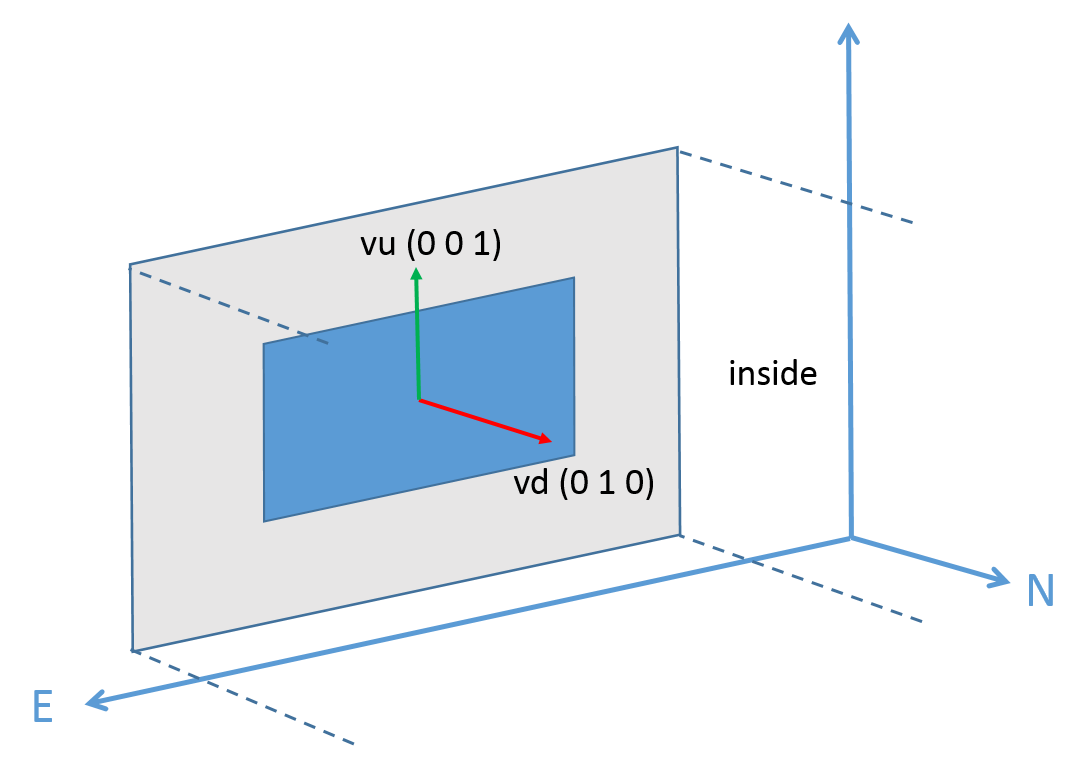
\includegraphics[width=1\textwidth]{windraw}
\end{minipage}
\quad
\begin{minipage}[c]{0.3\linewidth}
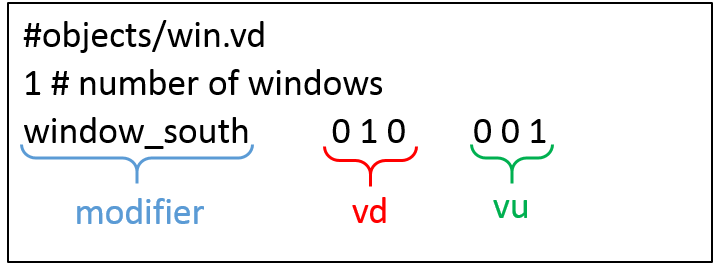
\includegraphics[width=1\textwidth]{winvd}
\end{minipage}
\caption{\label{img4:windoworient} New file with the list of windows in the scene and orientation of the vu and vd vectors}
\end{figure}

At the end you will have two files in the "window" folder, the win.vd and the window\_south.rad. Pay attention that the name \underline{window\_south} has to be the same for:
\begin{itemize}
\item *.rad file
\item window modifier within the *.rad file
\item window modifier within the win.vd file
\end{itemize}
as shown by the red rectangle in Figure \ref{img4:window_name}.

\begin{figure}[h]
\centering
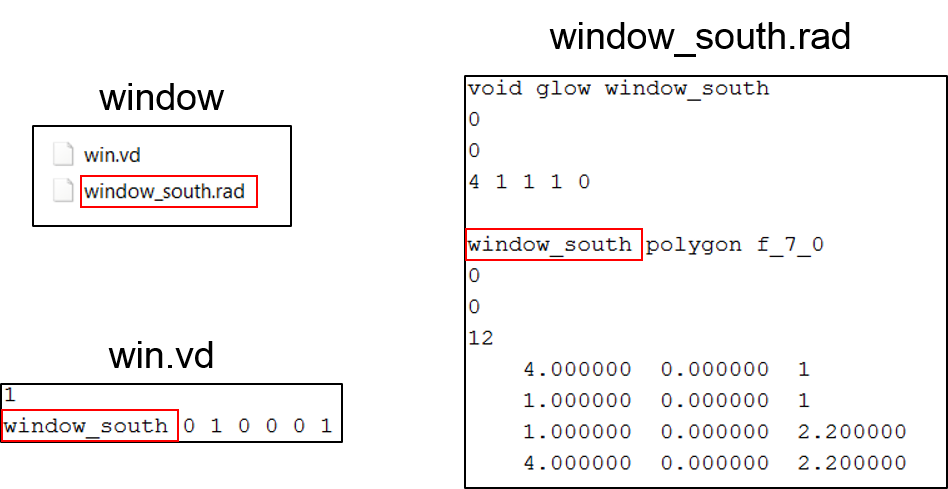
\includegraphics[width=0.7\textwidth]{window_name}
\caption{\label{img4:window_name} Correspondence on the window name within the several files}
\end{figure}

Delete some rows from the rad file that contains all the objects into the scene, Zone1.rad in this case (Figure \ref{img4:tutorial2}). In particular, the row that calls the sky definition and the window objects. In fact, TypeDLT creates at each time step a new sky file with the information contained in the weather file. And, the window/group of windows are used only for the matrices generations, during the simulations will be used the BSDFs data.

\begin{figure}[h]
\centering
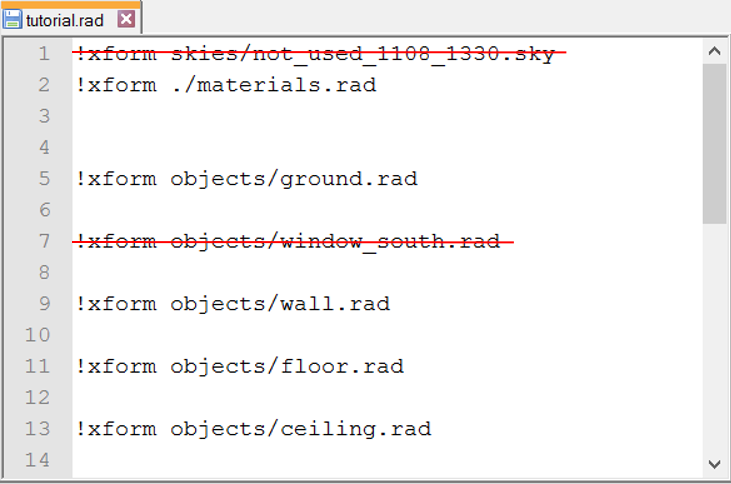
\includegraphics[width=0.6\textwidth]{tutorial2}
\caption{\label{img4:tutorial2} Contents of the tutorial.rad file}
\end{figure}

Finally, add the file containing the sensors grid within the \textit{data} folder with the the specific name {\color{blue}grid.pts}. The format to follow is: x, y, z, dx, dy, dz where x, y and z are the three dimensional coordinates of the point and dx,dy and dz are the coordinates of the vector that define view direction of the sensor.
The example file (figure \ref{img4:grid}) is composed by row grid with 9 sensors located in the middle of the scene 1 meter from the window with a step of 0.5 m.

\begin{figure}[h]
\centering
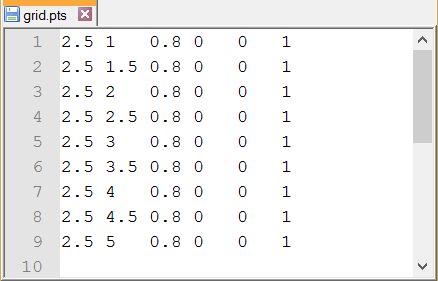
\includegraphics[width=0.5\textwidth]{grid}
\caption{\label{img4:grid} Format of the file containing the sensors grid}
\end{figure}

\section{Checking of the surface normal direction} \label{sec:normalsurf}

Before starting the simulations it is necessary to verify the right orientation of the window towards the inside of the room.
To do this follow this procedure: 
\begin{enumerate}
\item Open the command prompt of Windows following the steps:
\begin{itemize}
\item Type WinKey + R
\item Input "cmd"
\item Type Enter
\end{itemize}
\item Move into the Zone1 folder within the command prompt. Type "cd" (change directory) followed by the path of the Zone1 folder  in the command line 
\begin{center}
cd path\textbackslash of\textbackslash folder\textbackslash Zone1
\end{center}

\item Create a binary file containing the whole scene writing in the terminal the command 
\begin{center}
oconv materials.rad Zone1.rad window\textbackslash window\_south.rad > temp\textbackslash model.oct
\end{center}
this command converts the text format file of the scene in a binary format file readable by the Radiance functions. Change the name of the window rad files according to your model. Radiance requires to list the materials.rad files always before the geometry (Zone1.rad) it modifies, in your next simulations please follow this sequence in order to avoid errors during this initial step.

\item  Last step, create a preview of the room and check that the surface normal faces the correct direction with the command 
\begin{center}
rvu -ab 2 -vf views\textbackslash south\_view.vf -av 0.2 0.2 0.2 temp\textbackslash model.oct
\end{center}
where ab (ambient bounce) identifies the number of light reflections within the scene; av (ambient value) is used to set the overall light level in the scene, using a value of 0.2 (the three values regard the channels RGB) gives the possibility to see the inside of room even though the surface normal face the incorrect direction (figure \ref{img4:rvublack}). 
\end{enumerate}

If the surface is correctly oriented we will see a white light emitted from the window polygon (figure \ref{img4:rvu}), otherwise we will look at a black room (figure \ref{img4:rvublack}). This because the light material glow emits light only in the direction of the surface normal. \\
In the second case, black room, will be necessary reverse the surface normal. It can be done in SketchUp dropping the cursor on the surface to be reversed, right click on the surface and select \textit{Reverse Faces}. At this point export the window, with the procedure explained in section \ref{sec:export}, replace it with the incorrect one and run again the test.


\begin{figure}[h] 
\centering
  \subfigure[Surface normal correct direction]{% 
    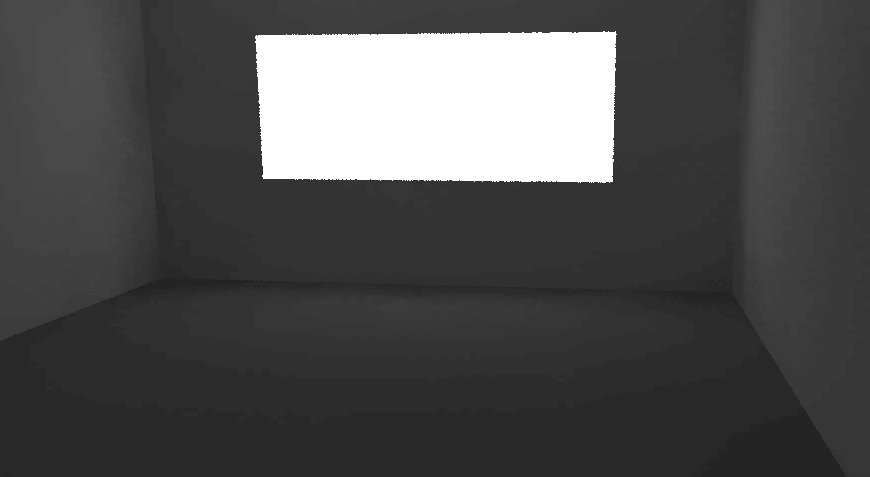
\includegraphics[width=.7\textwidth]{rvu} \label{img4:rvu} 
  } 
  \subfigure[Surface normal incorrect direction]{% 
    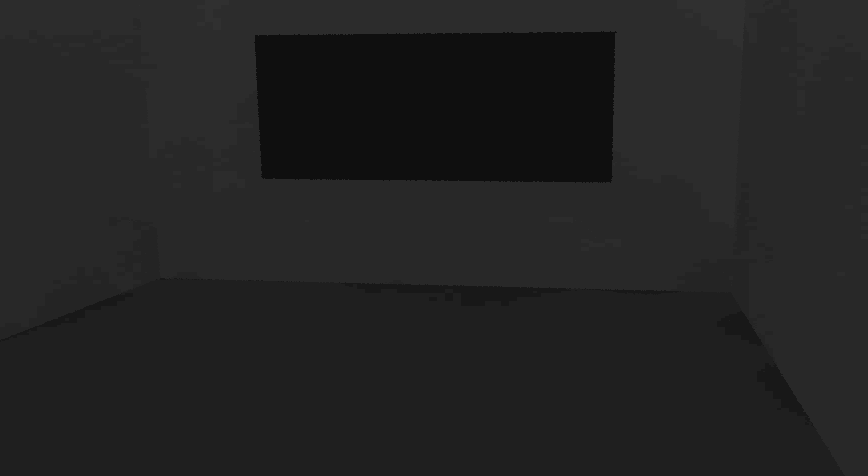
\includegraphics[width=.7\textwidth]{rvublack} \label{img4:rvublack} 
  }
  \caption{\label{img4:surfacenormal} rvu rendering of the inside room without and with light emitting window polygon }
\end{figure}
 




